\chapter{Final Project}


%%%%%%%%%%%%%%%%%%%%%%%%%%%%%%%%%%%%%%%%%%%%%%%%%%%
%                  0.
%%%%%%%%%%%%%%%%%%%%%%%%%%%%%%%%%%%%%%%%%%%%%%%%%%%
\section{Introdution}
Geological Carbon Storage (GCS) is an important technology to store the used carbon resources produced by burning fossil fuels,
and avoid the damaging consequences of climate change. 
A range of observations suggests that geological carbon storage is much less risky than unabated carbon emissions to the atmosphere.
\citep{bickle2009geological}


There are some ways to store carbon dioxide, for example, pumping carbon dioxide into a suitable geological reservoir, depleted oil and gas reservoirs.
Some cases also pumped carbon dioxide into saline aquifers underground, the deep ocean or onto the sea bed \citep{KOLSTER201877}.
However, most of the strategies raise safety concerns, practicality, the $CO_2$ leakage.
Figure ~\ref{fig:gcs}  \citep{gatech} shows an illustration of different leakage scenarios of Geological Carbon Storage.

\begin{figure}[H]
    \centering
    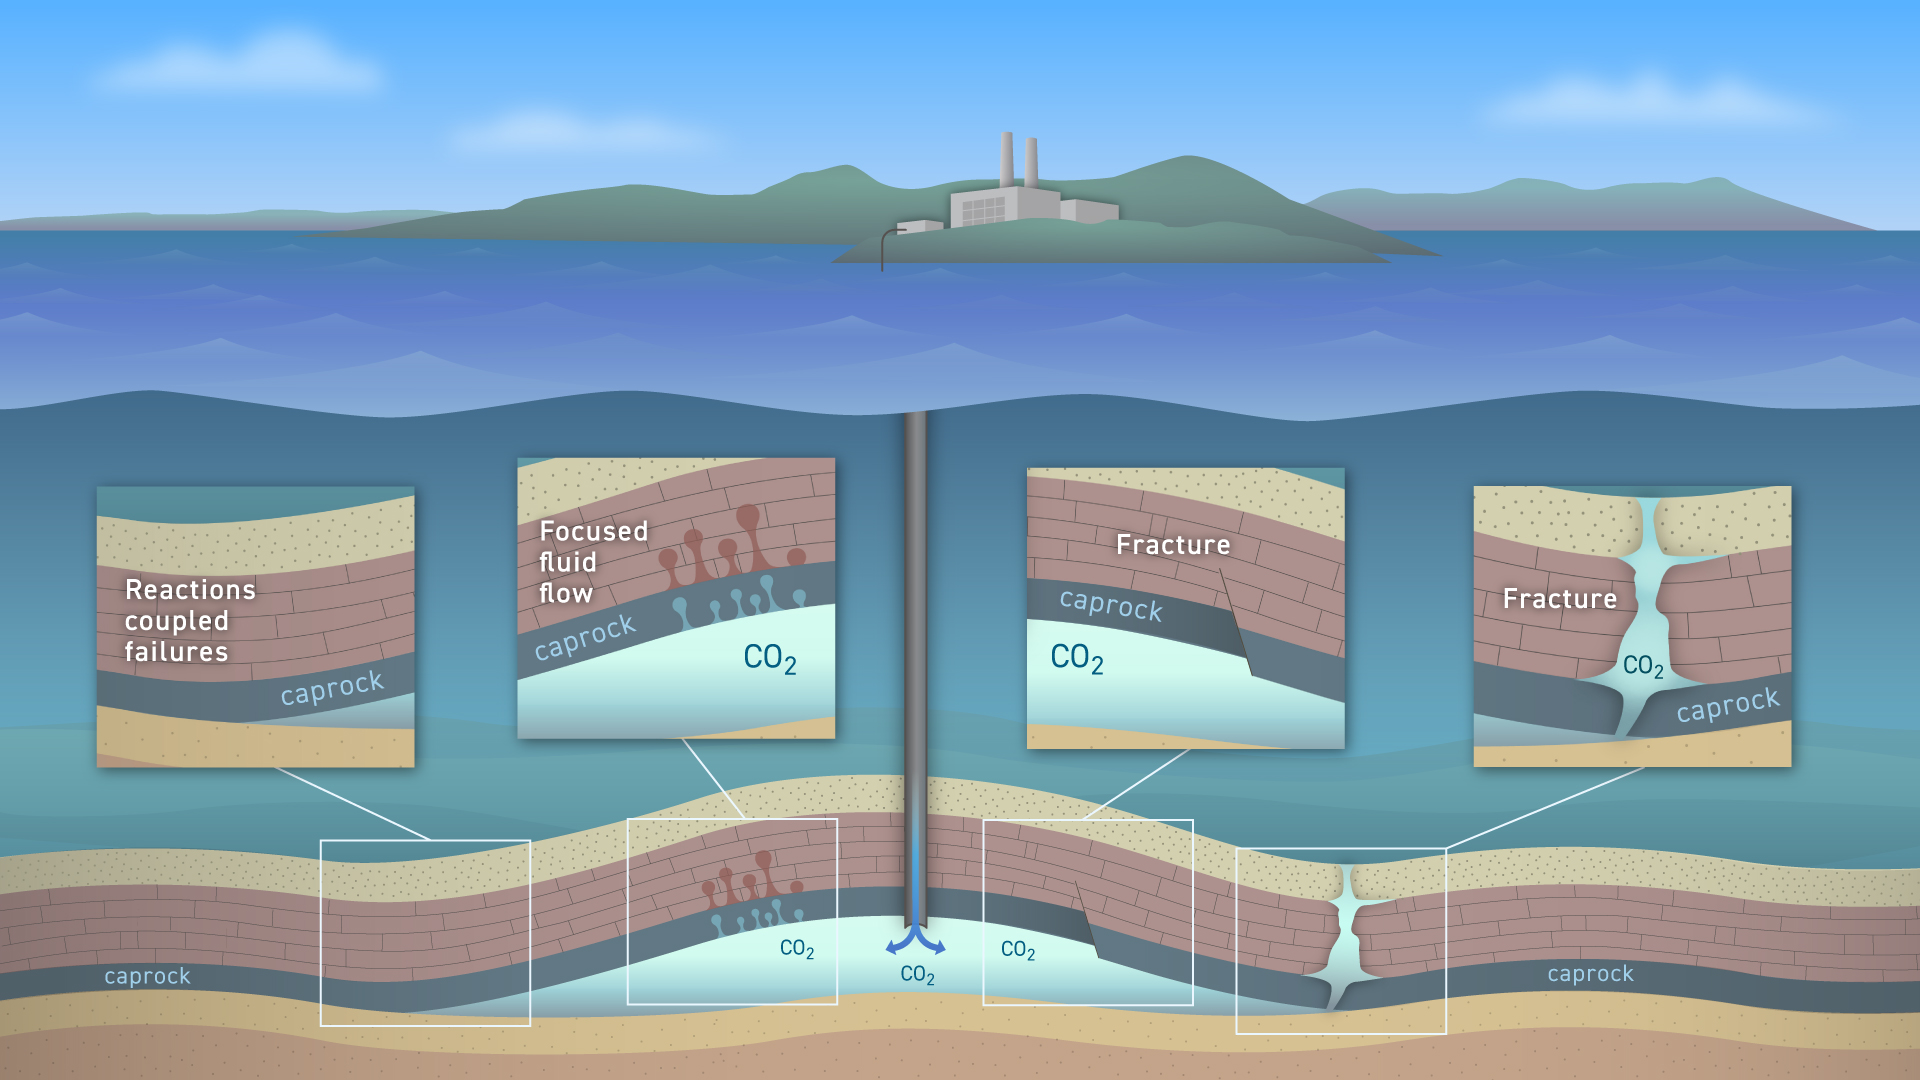
\includegraphics[width=0.7\textwidth]{figures/project/gcs.png}
    \caption{Illustration of Geological Carbon Storage}
    \label{fig:gcs}
\end{figure}

Figure out the mechanism of $CO_2$ migration is the first step to monitor Geological Carbon Storage.
In the next parts, I have made two simulation of $CO_2$ injecting to analyze the detail features.


%%%%%%%%%%%%%%%%%%%%%%%%%%%%%%%%%%%%%%%%%%%%%%%%%%%
%                  1.
%%%%%%%%%%%%%%%%%%%%%%%%%%%%%%%%%%%%%%%%%%%%%%%%%%%

\section{Data}

The velocity model showing in figure ~\ref{fig:Velocity_Model},
is downloaded from the following link, 
and the model is representative of the geology in the southeast of the North Sea, 
an area currently considered for carbon sequestration \citep{yin2021compressive}.

\href{https://www.dropbox.com/s/tksm9e2w4opj9ib/Compass2km.jld2}{https://www.dropbox.com/s/tksm9e2w4opj9ib/Compass2km.jld2}

According to the UK CCS Storage Appraisal Project's report \citep{UKreport2016},
the stratigraphic profile can be roughly divided into three parts:
on the bottom is the main reservoir location, made of high permeable sandstones (>200mD);
the 50m-depth primary seal lays over the reservoir, made of low permeable Rot Halite member ($10^{-3}$mD);
a secondary seal is above the primary seal, made of relatively low permeable Haisborough group (15-20mD) \citep{yin2021compressive}.

\begin{figure}[H]
    \centering
    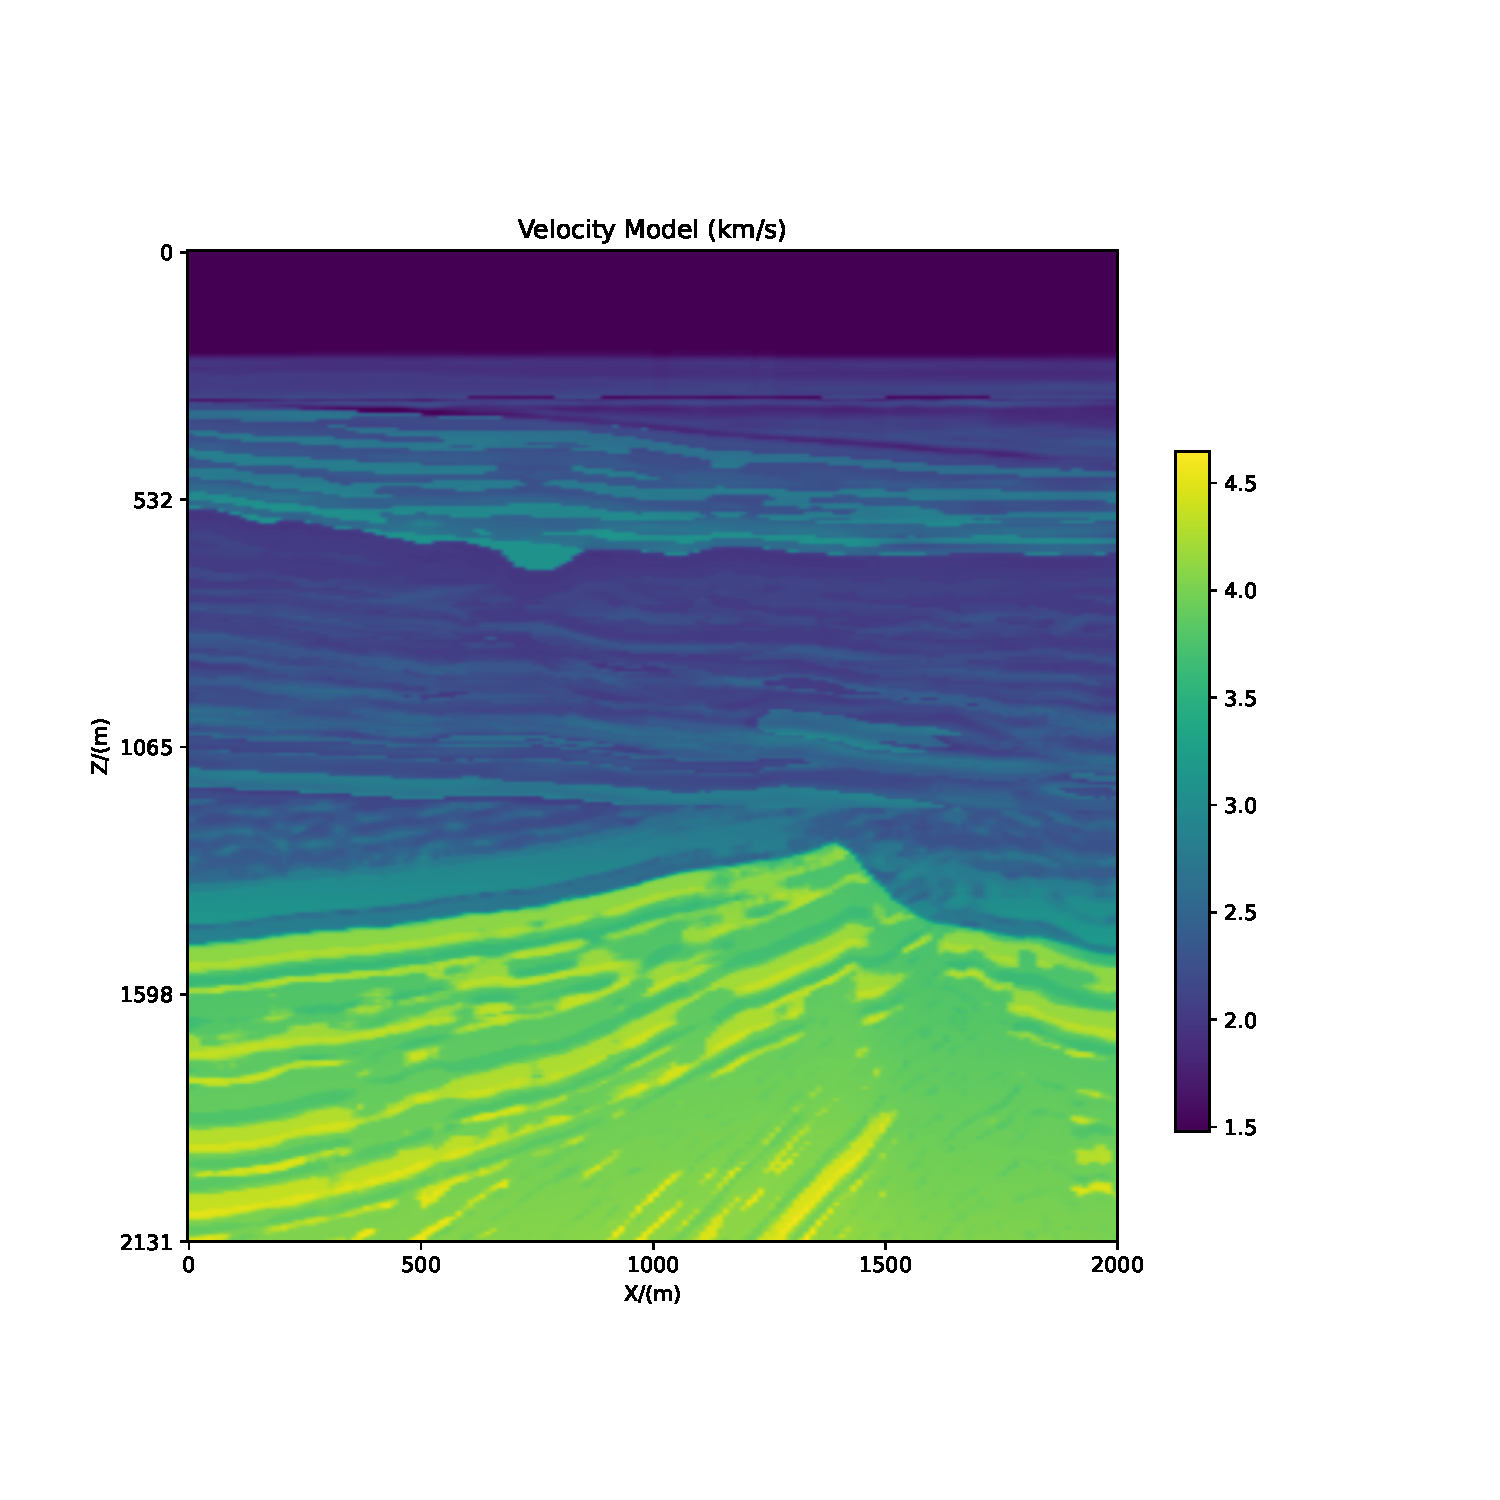
\includegraphics[width=0.7\textwidth]{figures/project/Velocity_Model.pdf}
    \caption{Velocity Model}
    \label{fig:Velocity_Model}
\end{figure}

In each region, I assume a linear relationship between seismic velocity and permeability, 
indicated by the paper \citep{klimentos1991effects} , where an increase of 1 km/s in velocity corresponds to an increase of 1.03mD in permeability.
The permeability model is showing in figure ~\ref{fig:Permeability_Model}

\begin{figure}[H]
    \centering
    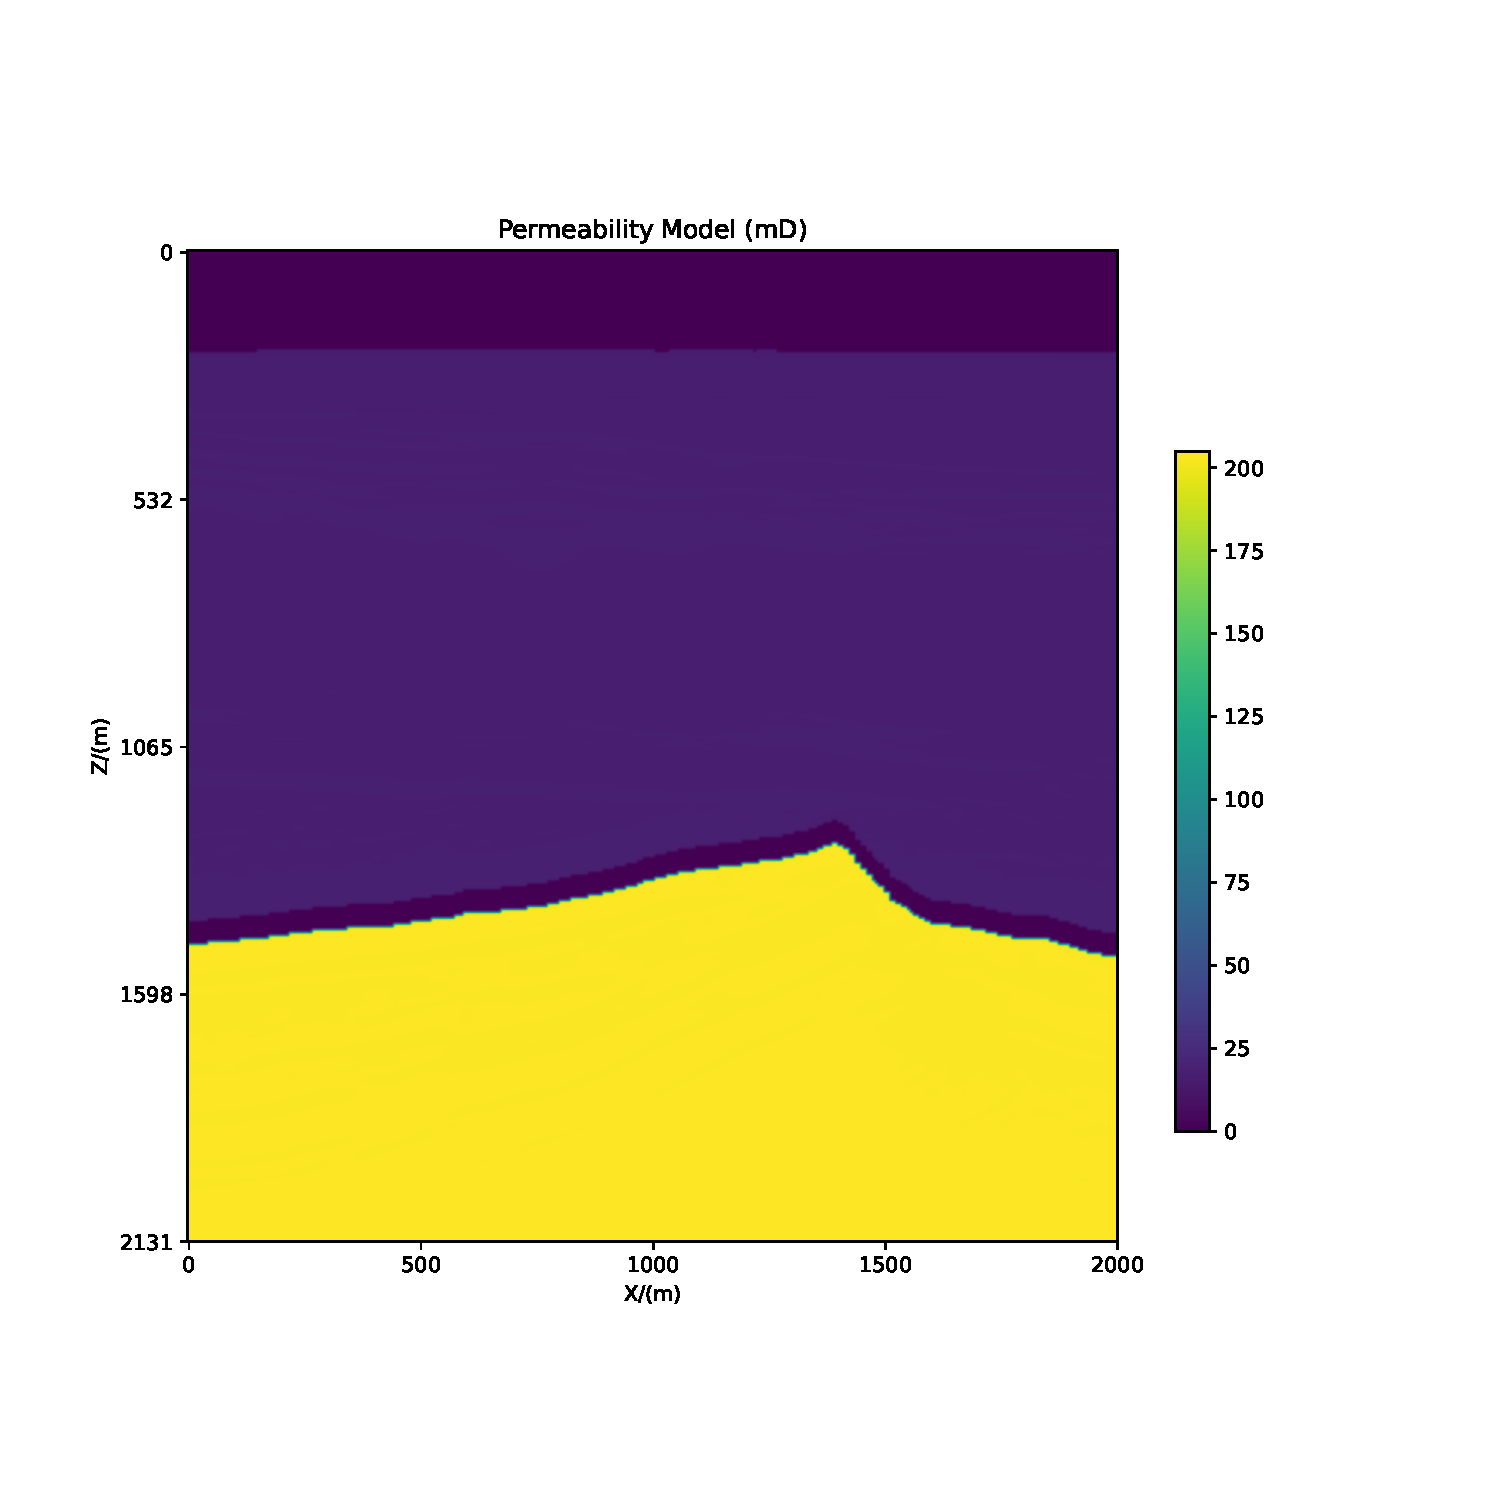
\includegraphics[width=0.5\textwidth]{figures/project/Permeability_Model.pdf}
    \caption{Permeability Model}
    \label{fig:Permeability_Model}
\end{figure}

Then according to the paper \citep{costa2006permeability}, I convert the permeability model to porosity model via
Kozeny-Carman relationship, and the formula is showing below and the values are taken from Strategic UK CCS Storage Appraisal Project \citep{UKreport2016}:

\begin{align}
    K = \phi^3 {( \frac{ 1.527 }{ 0.0314*(1-\phi)} )}^2
    \label{equ:KC}
\end{align}


Where $\phi$ is porosity and $K$ is permeability. The porosity model is showing in figure ~\ref{fig:Porosity_Model}

\begin{figure}[H]
    \centering
    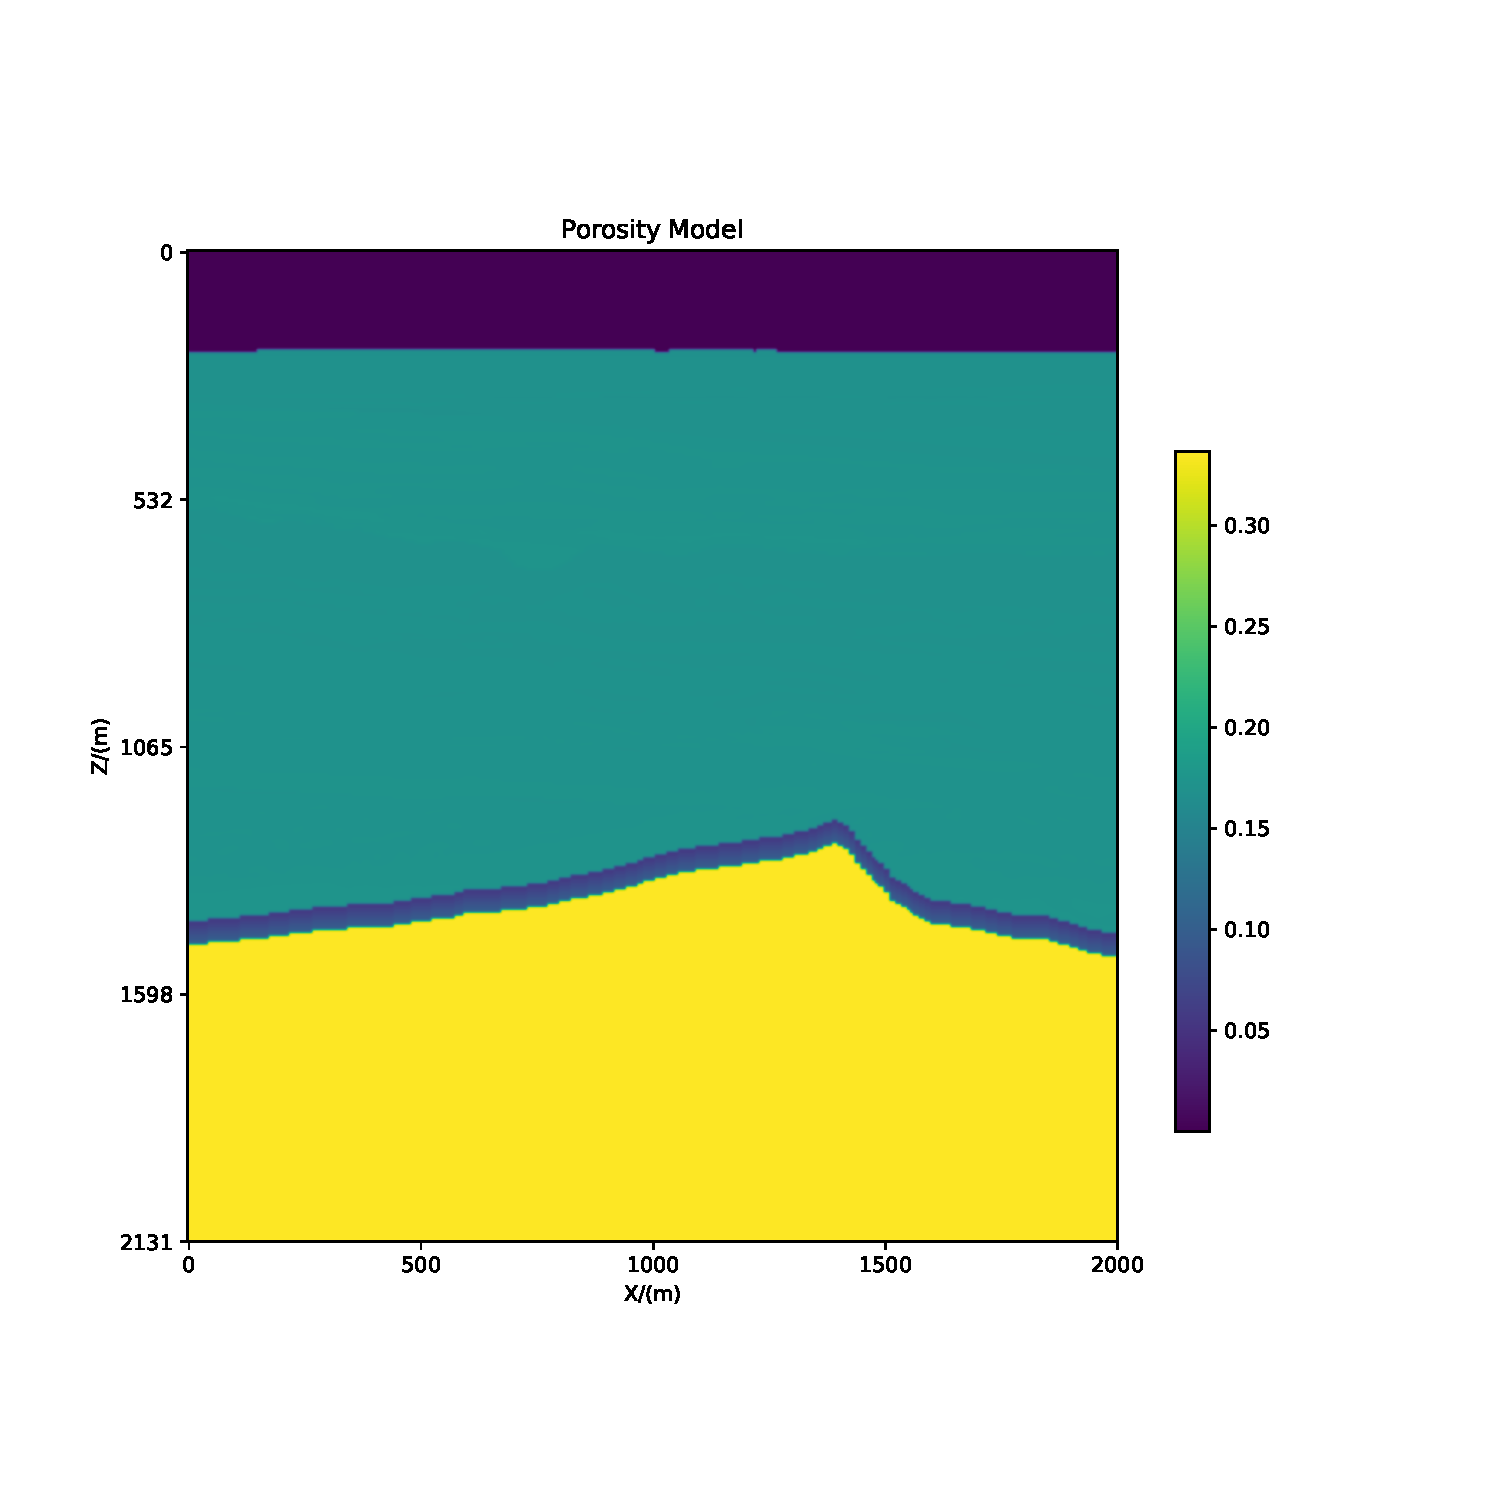
\includegraphics[width=0.5\textwidth]{figures/project/Porosity_Model.pdf}
    \caption{Porosity Model}
    \label{fig:Porosity_Model}
\end{figure}


%%%%%%%%%%%%%%%%%%%%%%%%%%%%%%%%%%%%%%%%%%%%%%%%%%%
%                  2.
%%%%%%%%%%%%%%%%%%%%%%%%%%%%%%%%%%%%%%%%%%%%%%%%%%%
\section{Method}

For two-phase flow simulation, I use the software FwiFlow \citep{li2020coupled} to simulate the growth of 
$CO_2$ plume with a 2-D model. It mainly solves the flow equation by Newton-Raphson method.
The governing equation is derived from conservation of mass from each phase, we have:
\begin{align}
    \frac{\partial}{\partial t} (\phi S_i \rho_i) + \bigtriangledown \cdot (\rho_i v_i) = \rho_i q_i,   i=1,2
    \label{equ:flow1}
\end{align}


The saturation of the two phases satisfies
\begin{align}
    S_1 + S_2 = 1
    \label{equ:flow2}
\end{align}


and the Darcy's law yields
\begin{align}
    v_i = - \frac{K k_{ri}(S_i)}{u_i} (\bigtriangledown P_i - g \rho_i \bigtriangledown Z), i=1,2
    \label{equ:flow3}
\end{align}

where $K$ is the permeability tensor,$S_i$ is saturation, $k_{ri}(S_i)$ is the function of $S_i$,
$u_i$ is the viscosity, $Z$ is the depth, $\rho_i$ is the density, $\phi$ is the porosity,
$P_i$ is the fluid pressure, and $g$ is the velocity constant \citep{li2020coupled}.


The fluid pressure $P_i$ is related to $S_i$ via the capillary pressure
\begin{align}
    P_2 = P_1 - P_c(S_2)
    \label{equ:flow4}
\end{align}

And $P_c$ is a function of the saturation of the wetting phase 2.

After many experiments, I found that the growth of $CO_2$ plume is most sensitive to the permeability,
which means $CO_2$ mostly like to migrate to the areas with relatively large permeability value.
I will discuss this feature later.

I made a period simulation of almost six years with a time step of 20 days,
and the grid spacing is 6.25 $m$. The simulation results is showing in figure \ref{fig:CO2_Saturation1},
which have 9 snapshots from 1-st day to last day with equal time intervals.

We can clearly find how the plume develops over time under influence of buoyancy, where 
the red cross is the injected location. 
We found that $CO_2$  migrated upwards over time, eventually hitting caprock which has a very low permeability 
where $CO_2$  is almost impossible to penetrate through.
Then $CO_2$  moved to the two sides.
The areas where is near to the caprock has a high $CO_2$ saturation finally.



\begin{figure}[H]
    \centering
    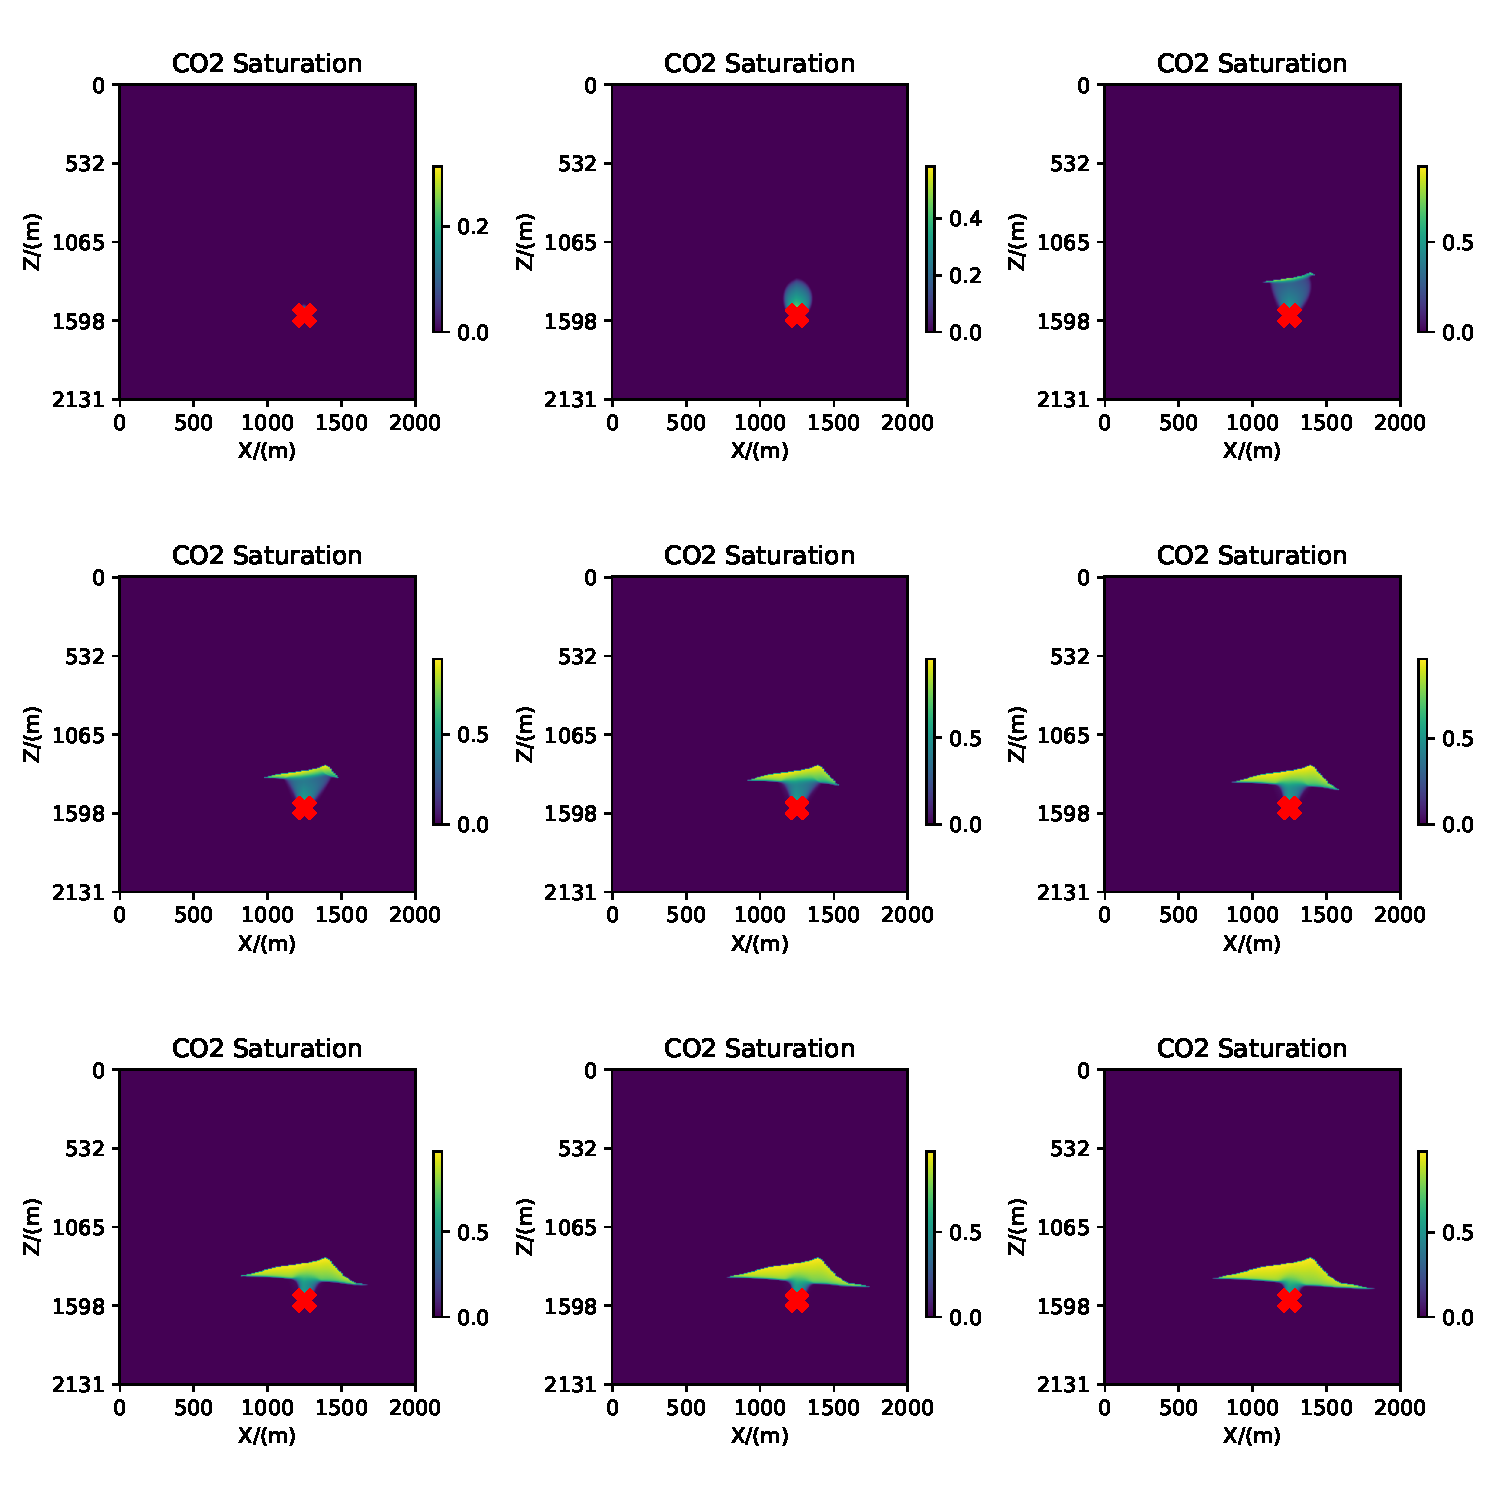
\includegraphics[width=0.95\textwidth]{figures/project/CO2_Saturation1.pdf}
    \caption{CO2 Saturation}
    \label{fig:CO2_Saturation1}
\end{figure}


The two flows properties can be found in table \ref{tab:flow properties}. I assumed that the pores
were filled with water firstly, and then replaced by $CO_2$ by injecting way.

\begin{table}[h]
    \centering
    \caption{Flow properties}
    \label{tab:flow properties}
    %\begin{tabular}{c|cccp{6em}p{3em}c}
    \begin{tabular}{m{4cm}<{\centering} m{4cm}<{\centering} m{4cm}<{\centering}}
        \toprule
           & Water & $CO_2$    \\

        \midrule
        Density ($kg/m^3$) &  1000 & 0.353  \\
        Viscosity ($10^{-5} Pa\cdot s$) & 89    & 1.372\\
        Bulk Modulus ($MPa$) &  2100  & 0.0258  \\

        \bottomrule
    \end{tabular}
\end{table}


%%%%%%%%%%%%%%%%%%%%%%%%%%%%%%%%%%%%%%%%%%%%%%%%%%%
%                  3.
%%%%%%%%%%%%%%%%%%%%%%%%%%%%%%%%%%%%%%%%%%%%%%%%%%%
\section{Results and Discussion}

After the $CO_2$ injecting simulation, I used the White and Dutta-Ode model \citep{lewandowski2009book} to analyze the
changes of velocity and attenuation, because when pore pressures cannot equilibrate, fluid flow will cause attenuation and dispersion of the seismic wave. 
I used the same parameters of  $CO_2$ simulation for patchy model.
In addition, I set the P-wave frequency to 100 $hz$, which controled the transfer of two
fluid phases in fluid boundaries.
And I used two patchy size: $2 cm$ and $5 cm$.

\begin{figure}[H]
    \centering
    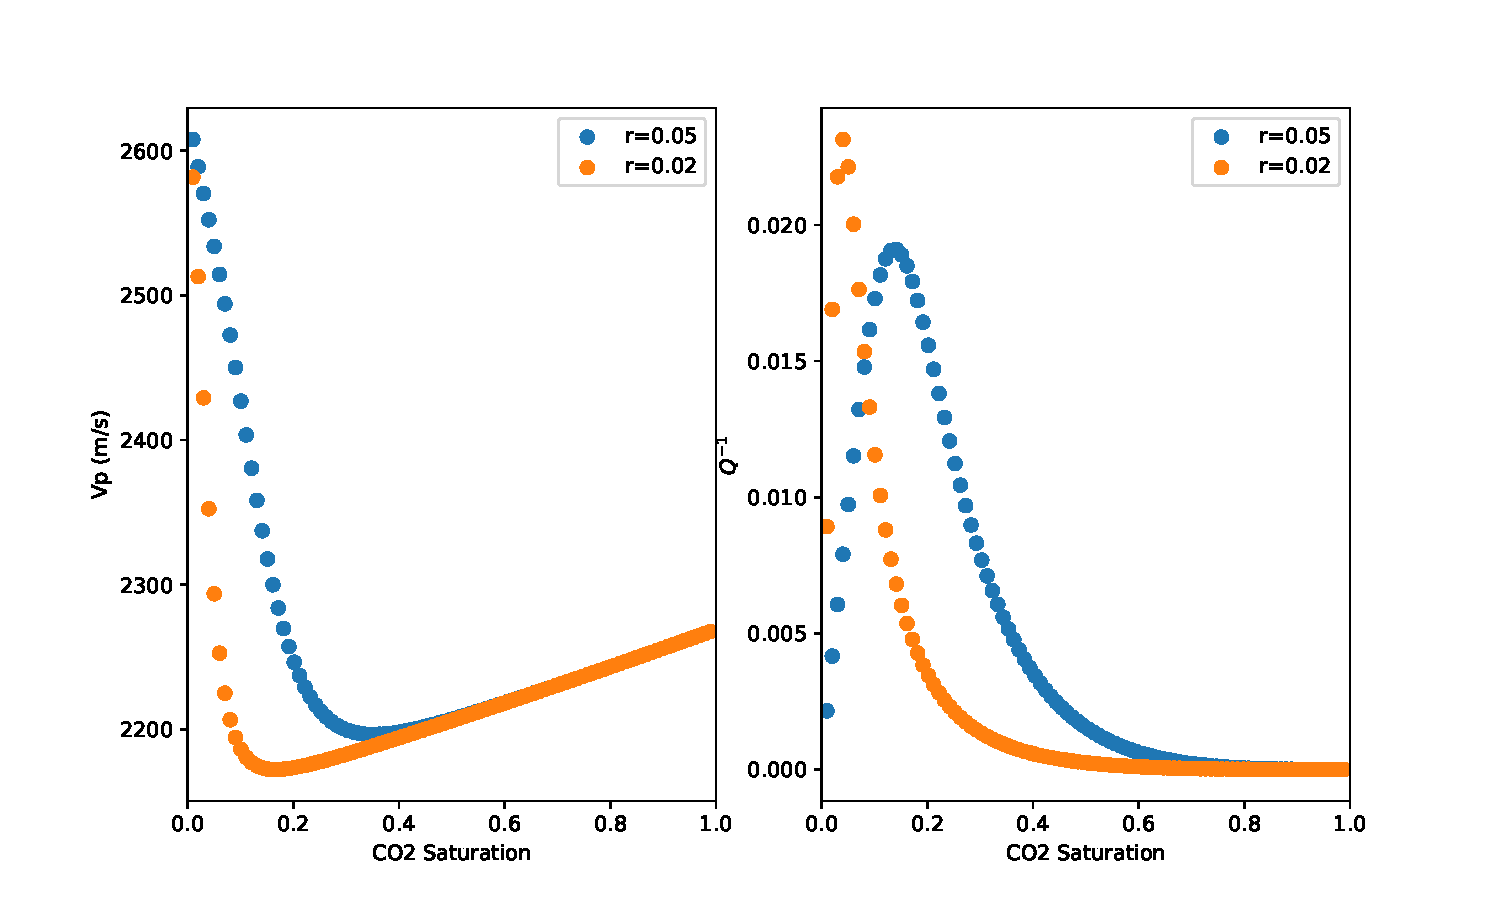
\includegraphics[width=0.9\textwidth]{figures/project/V_curve1.pdf}
    \caption{Velocity and attenuation curves with $CO_2$  saturation based on White and Dutta-Ode model}
    \label{fig:V_curve1}
\end{figure}


Figure \ref{fig:V_curve1} shows the results of P-wave velocity predicted from the White and Dutta-Ode model
as a function of saturation, and the raw velocity is around 2600 $m/s$ before $CO_2$ injection.
We can clearly find the P-wave velocity decreased as $CO_2$ saturation increased at the beginning, because
$CO_2$ is more compressible then water. And the drop value up to 450 $m/s$.
Large patchy size has a smaller velocity drop.
But when $CO_2$ saturation exceeds the critical point (the saturation is 0.15 for $2 cm$, 0.25 for $5 cm$ of patchy size),
the P-wave velocity will increase as $CO_2$ saturation increased, 
because of the density effect overtaking the bulk modulus effect.
And the increased value is around 100 $m/s$ which is smaller than the maximun drop value.
Those P-wave velocity changes are very large which can be easy detected by seismic imaging process.

For the changes of $Q^{-1}$ value, we can find it will increase firstly, and then decreased as a function of saturation.
The critical point is different for different patchy size, the saturation is 0.05 for $2 cm$ and 0.15 for $5 cm$ of patchy size.
Large patchy size has a smaller max $Q^{-1}$ value change.

Figure \ref{fig:V_change2Q} shows the 2-D model changes of velocity and attenuation with $CO_2$  saturation.
We found that the changes of P-wave velocity and $Q^{-1}$ value is appeared in place 
where $CO_2$ plume is present. 
But different from the conclusion above, the velocity is increased in those areas, maybe because
it greatly increased the density effect overtaking the bulk modulus effect. 
But this is against the common sense, it maybe that I used the wrong parameters to calculate 
dry bulk and dry shear modulus.

\begin{figure}[H]
    \centering
    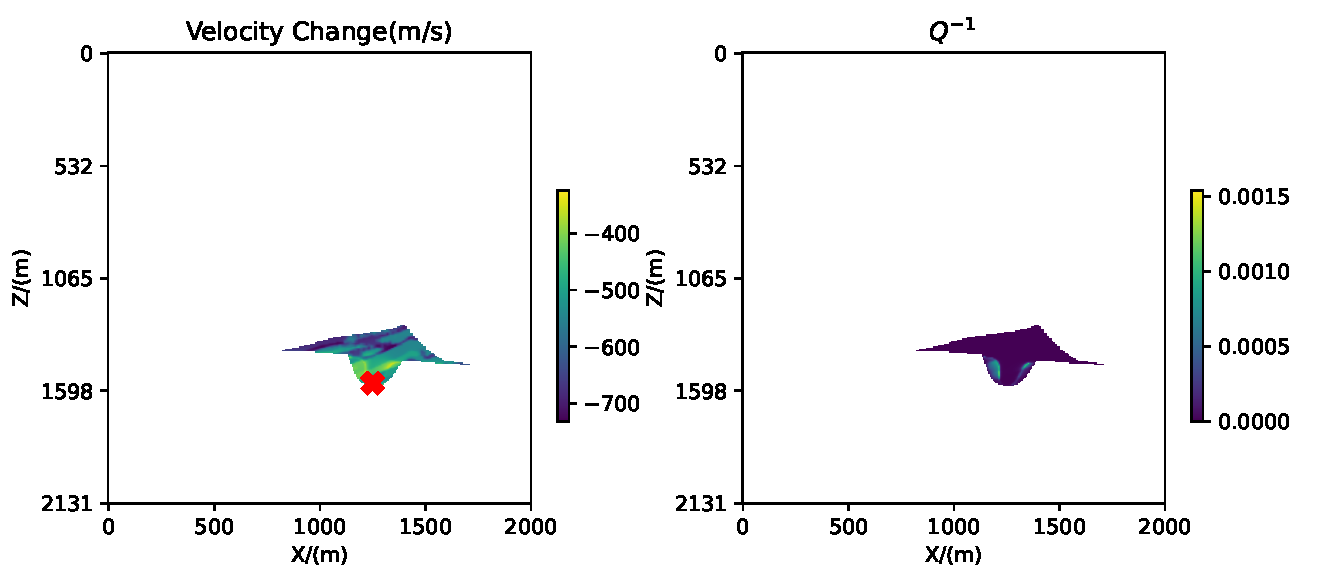
\includegraphics[width=0.9\textwidth]{figures/project/V_change2Q.pdf}
    \caption{The changes of velocity and attenuation model with $CO_2$  saturation based on White and Dutta-Ode model}
    \label{fig:V_change2Q}
\end{figure}





%%%%%%%%%%%%%%%%%%%%%%%%%%%%%%%%%%%%%%%%%%%%%%%%%%%
%                  4.
%%%%%%%%%%%%%%%%%%%%%%%%%%%%%%%%%%%%%%%%%%%%%%%%%%%
\section{What will happen if $CO_2$ leaked?}

The first simulation is an example well-stored $CO_2$. I also want to know what will happen
if $CO_2$ leaked? So I DIY a small model, the velocity and density model is showing in figure \ref{fig:vel_density},
the permeability and porosity model is showing in figure \ref{fig:pere_poro}.

The red cross is the injection location.
I set a fault near to the injection point, and about 30 meters above is a caprock layer with very low permeability.
This simulation has the same  parameters of flud properties with 1-st simulation.
The time period of simulation is almost six years with a time step of 20 days,
and the grid spacing is 6 $m$. 

Figure \ref{fig:CO2_Saturation2} shows the results of CO2 saturation, which have 9 snapshots from 1-st day to last day with equal time intervals.
And we can find 
$CO_2$ first migrates and diffuses under the caprock, then migrates to the top of the caprock through faults channel, 
eventually migrates to most of the space.
Although the permeability and porosity is larger above the caprock, 
but the $CO_2$ saturation is smaller than the areas below the caprock,
which may be  due to the inefficient leakage through the small fault.



\begin{figure}[H]
    \centering
    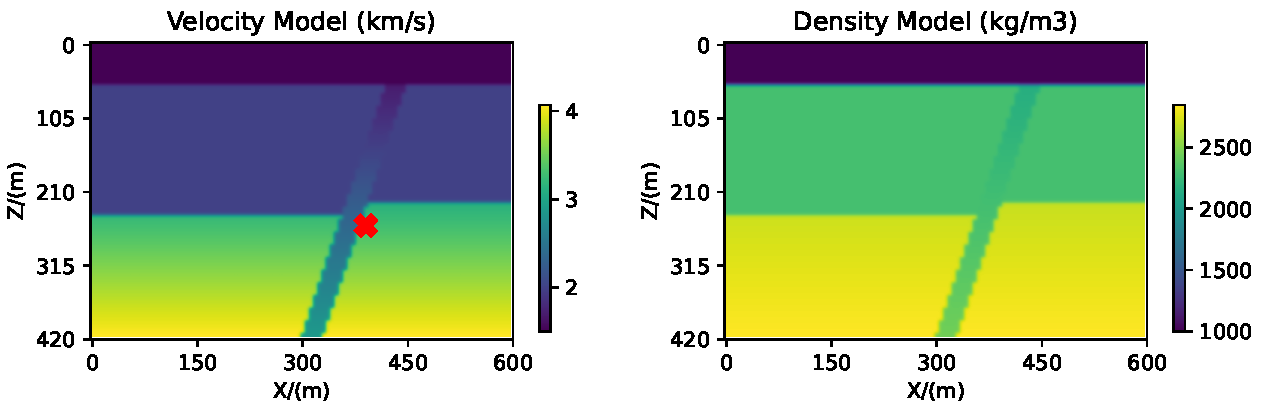
\includegraphics[width=0.9\textwidth]{figures/project/vel_density.pdf}
    \caption{Velocity and Density Model}
    \label{fig:vel_density}
\end{figure}



\begin{figure}[H]
    \centering
    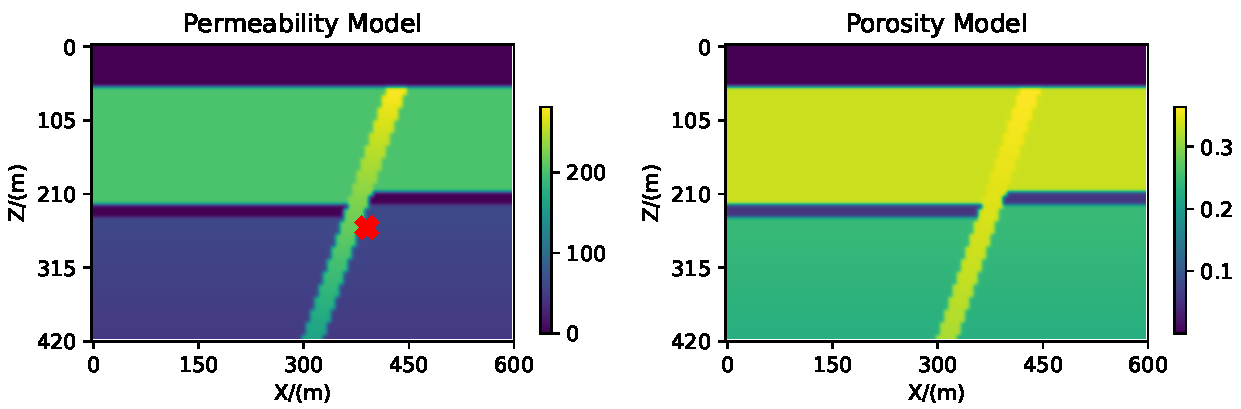
\includegraphics[width=0.9\textwidth]{figures/project/pere_poro.pdf}
    \caption{Permeability and Porosity Model}
    \label{fig:pere_poro}
\end{figure}



\begin{figure}[H]
    \centering
    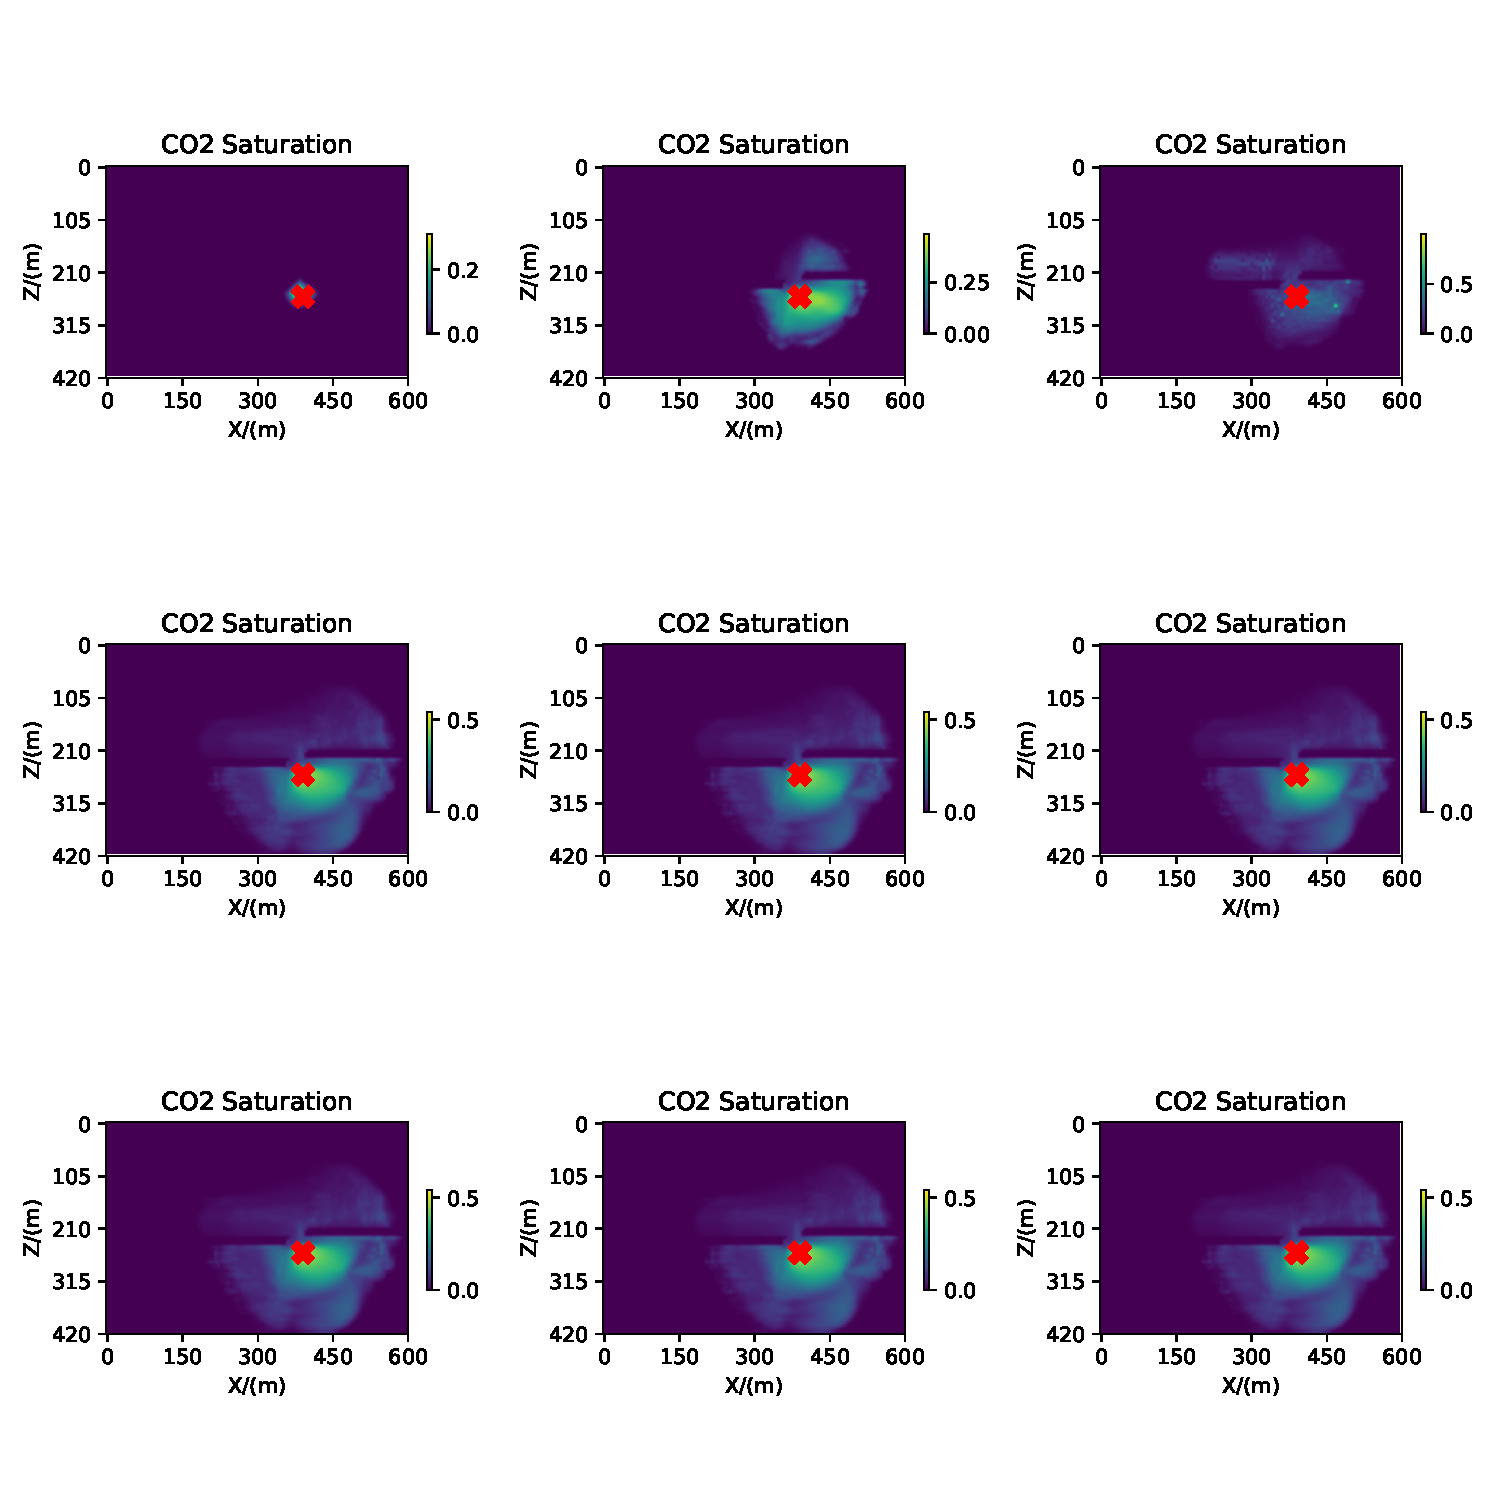
\includegraphics[width=0.9\textwidth]{figures/project/CO2_Saturation2.pdf}
    \caption{CO2 Saturation}
    \label{fig:CO2_Saturation2}
\end{figure}

%%%%%%%%%%%%%%%%%%%%%%%%%%%%%%%%%%%%%%%%%%%%%%%%%%%
%                  5.
%%%%%%%%%%%%%%%%%%%%%%%%%%%%%%%%%%%%%%%%%%%%%%%%%%%
\section{Scripts}
The project mainly include 7 scripts.
If you want to run the codes, make sure you have install the following packages: numpy, matploltib, h5py, julia, NPZ.jl, JLD2.jl, FwiFlow.jl, Seis4CCS.jl.
And the FwiFlow package can only be run via GPU (for example you can run it on NOTS cluster).

\subsection{01\_run.jl}
\juliafile{figures/project/01_run.jl}

\subsection{01\_plot.py}
\pythonfile{figures/project/01_plot.py}

\subsection{02\_model.py}
\pythonfile{figures/project/02_model.py}

\subsection{02\_run.jl}
\juliafile{figures/project/02_run.jl}

\subsection{02\_plot.py}
\pythonfile{figures/project/02_plot.py}

\subsection{PatchyWhite.py}
\pythonfile{figures/project/PatchyWhite.py}

\subsection{utilize.jl}
\juliafile{figures/project/utilize.jl}

\clearpage